\chapter{Developer Documentation}

The implementation of the NextGen SPICE library is contained in one Visual Studio 2017 solution which consists of 10 projects; the overall structure of the solution is illustrated in figure~\ref{fig:solution-structure}.

\begin{figure}[h]
	\centering
	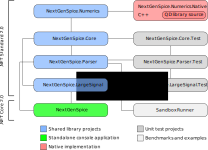
\includegraphics[width=0.87\linewidth]{solution-structure}
	\caption{Project structure of the solution}
	\label{fig:solution-structure}
\end{figure}

The \texttt{NextGenSpice.Core} project is the core project of the library, it contains classes for creating and validating electrical circuits. It also contains code that automatically discovers available analysis types through the MEF framework, and constructs analysis-specific circuit models from circuit description.

The \texttt{NextGenSpice.LargeSignal} project contains the implementation of the large-signal circuit model which allows performing DC operating point and transient analyses.

The \texttt{NextGenSpice.Parser} project contains the implementation of the SPICE netlist parser and allows users of the library to import circuits, subcircuits and device model parameters into the simulator.

The \texttt{NextGenSpice.Numerics} project defines classes for creating and representing equation systems for the simulator, as well as other mathematical functions that are needed in the simulator. It also serves as a managed wrapper around the \texttt{NextGenSpice.Numerics.Native} C++ project, which is used to build the QD library for double-double and quad-double arithmetic, and expose its methods to managed (C\#) code.

\texttt{NextGenSpice} represents the standalone console application, the implementation of which was the goal~\ref{goal:app} of this thesis. It is also the only library project which targets the .NET Core platform.

The other projects are not part of the distributed library or console application. The \texttt{SandboxRunner} console application project is used to run benchmarks for the circuit simulator, and the projects with \texttt{.Test} suffix contain unit tests for individual parts of the library.

\subsubsection{License}
The whole NextGen SPICE solution is provided under the MIT license. More details can be found in the \texttt{LICENSE.TXT} file in the solution folder (located in the \texttt{/sources} folder in the attached CD).

\section{Compilation}

To allow using enhanced precision types in the simulator library, the solution contains one C++ project (\texttt{NextGenSpice.Numerics.Native}), which potentially inhibits the portability of the library. As discussed in analysis section~\ref{chap:analysis:dd}, we decided that the use of C++ code should be conditional on the presence of compile time symbols. The use of native code depends on the conditional compilation symbols used when compiling the \texttt{NextGenSpice.Numerics} project. In Visual Studio 2017, these symbols can be set in Project Properties $\rightarrow$ Build $\rightarrow$ Conditional compilation symbols. The following table lists the symbols and their meaning for the compilation.


\newcolumntype{L}{>{\centering\arraybackslash}m{10cm}}
\begin{center}
	\begin{tabular}{|c|L|}
		\hline 
		Symbol & Precision type used \\ \hline \hline
		\texttt{dd\_precision}& Use the \texttt{dd\_real} type and double-double arithmetic \\ \hline 
		\texttt{qd\_precision}& Use the \texttt{qd\_real} type and quad-double arithmetic \\ \hline 
		\textit{no symbol} & Use the \texttt{double} type \\ \hline 
	\end{tabular}
\end{center}

\begin{center}
	\begin{tabular}{|c|L|}
		\hline 
		Symbol & Choice of Gauss elimination implementation \\ \hline \hline
		\texttt{native\_gauss}& Use native implementation  \\ \hline 
		\textit{no symbol} & Use managed implementation \\ \hline 
	\end{tabular}
\end{center}

The \texttt{NextGenSpice\+.Numerics\+.Native.dll} dll is defaultly compiled for 64-bit runtime. To use NextGen SPICE library in a 32-bit process, a 32-bit version of the  native dll must be compiled.

\section{NextGenSpice.Core}

The \texttt{NextGenSpice.Core} assembly contains the analysis independent parts of the NextGen SPICE library, namely the classes for circuit description, logic for validating the circuit, and a generic factory to be used for creating analysis-specific circuit models.

\subsection{Circuit Description}

In the analysis section~\ref{fig:analysis:representation-circuit}, we decided to represent the circuit description using a separate class for each device. These classes implement the \texttt{ICircuitDefinition\+Device} which defines the members \texttt{ConnectedNodes} and \texttt{GetBranchMetadata} which are used to validate the circuit topology. It also defines members \texttt{Tag} which can be used to identify individual devices and a \texttt{Clone} method for duplicating the device.

The \texttt{ConnectedNodes} property returns an instance of the \texttt{NodeConnectionSet} class which encapsulates the node connections. This class has \texttt{internal} setters, so that the connections are set only by the library and cannot be modified by the user.

\texttt{GetBranchMetadata} is used to retrieve the characteristics of the connections which are important for the circuit topology validation. The topology rules require that there is no cycle of voltage sources and inductors, and no cutset of current sources and capacitors. \texttt{GetBranchMetadata} therefore returns a collection of \texttt{CircuitBranchMetadata}  which contain information whether the device is \textit{current defined} or \textit{voltage defined}. If a device is neither (e.g.\ resistor), then the \texttt{GetBranchMetadata} returns an empty collection.

The circuit description is contained in the \texttt{CircuitDefinition} class, which simply wraps collection of \texttt{ICircuitDefinitionDevice} and provides other convenient methods (such as \texttt{FindDevice} to find a device by its tag). This class also has \texttt{internal} constructors, so that it can be created only by the library's code. The circuit definition is created by the \texttt{CircuitBuilder} class, which is also responsible for validating the circuit's topology.

The SPICE subcircuit representation consists of two parts: a \texttt{Subcircuit\+Definition} class which contains the description of the subcircuit in a similar manner as the \texttt{CircuitDefinition} class, and the \texttt{Subcircuit} class which implements the \texttt{ICircuitDefinitionDevice} interface and represents the subcircuit usage in the circuit. The \texttt{Subcircuit\+Definition} instances are shared among all coresponding \texttt{Subcircuit} classes.

\subsection{General Analysis Implementation Design}

Before we cover the mechanism which creates the analysis-specific circuit models from the circuit description, we will describe the interface hierarchies between the circuit description and analysis implementation. The \texttt{ICircuitDefinition} and \texttt{ICircuitDefinitionDevice} interfaces were described in previous subsection. The interfaces on the analysis implementation counterparts are \texttt{IAnalysis\+CircuitModel<TDevice>} and \texttt{IAnalysisDeviceModel<TAnalysis>}.

Because the relationship between these two interfaces is not trivial, we will explain them in the context of the large-signal analysis model implementation. Figure~\ref{chap:devdocs:analysis-design} shows the relationship between the classes and interfaces for circuit description and the large-signal circuit model.

\begin{figure}[h]
	\centering
	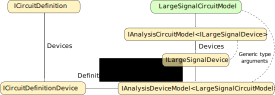
\includegraphics[width=.8\linewidth]{analysis-interface}
	\caption{Connection between the circuit description and analysis implementation}
	\label{chap:devdocs:analysis-design}
\end{figure}

The implementations of concrete analysis types are expected to extend the \texttt{IAnalysisDeviceModel} interface by adding methods required from the device's implementation. The additional methods for large-signal analysis are defined in \texttt{ILargeSignalDevice} which extends the \texttt{IAnalysisDeviceModel<LargeSignal\+CircuitModel>} interface. The generic argument in the \texttt{IAnalysisDeviceModel} interface is not used in the defined members, but provides metadata useful for enforcing that only the classes implementing \texttt{ILargeSignalDevice} interface can be registered as device models for \texttt{LargeSignalCircuitModel} (the model registration and analysis model factories will be covered in a later subsection). The \texttt{IAnalysisDevice\+Model} interface defines the \texttt{DefinitionDevice} property which serves as the link to the device from the original circuit description. The classes implementing the device-specific simulation logic will read the device's parameters from its definition device, which allows reacting to the changes of the device's parameters, as requested by goal~\ref{goal:transient}.

The \texttt{IAnalysisCircuit\+Model} interface has a generic parameter for the base type of the device's implementation, which is also the type of the items in its \texttt{Devices} property. The \texttt{LargeSignalCircuitModel} class requires each device to implement the \texttt{ILargeSignalDevice} interface. 

%The \texttt{TDevice} generic parameter must implement the \texttt{IAnalysisDeviceModel<IAnalysisCircuitModel<TDevice>>} interface, which enforces the fact that only

\subsection{Analysis Model Creation}

The creation of analysis-specific circuit models is done via a set of factories. Each analysis type assembly  (currently, only \texttt{NextGenSpice.LargeSignal} is implemented) exports an implementation of \texttt{IAnalysisModelFactory<T>} specialized on the class which will be used to represent the circuit for the particular analysis. In the case of \texttt{NextGenSpice.LargeSignal}, the class \texttt{LargeSignalAnalysisModel\+Factory} implements the \texttt{IAnalysisModelFactory<Large\+SignalCircuitModel>} interface and is used to build \texttt{LargeSignalCircuitModel} instances.

The core functionality for registering models for individual circuit devices is implemented in the abstract \texttt{AnalysisModelFactory<T>} class. The registering is done by calling the generic method \texttt{SetModel<TDesc, TImpl>} specialized on a definition device type and implementation device type. This function takes a factory function as a parameter, which will be later used to construct the implementation class. For example, the registering of \texttt{LargeSignal\+Resistor} as the implementation for \texttt{Resistor} device is done by calling

\begin{csharpcode}
IAnalysisModelFactory<LargeSignalCircuitModel> factory = /*...*/;
factory.SetModel<Resistor, LargeSignalResistor>(
	e => new LargeSignalResistor(e));
\end{csharpcode}

Thanks to the interface definitions as described in the previous section, it is possible to constrain the type arguments of the \texttt{SetModel} method to statically check that the \texttt{LargeSignalResistor} class implements \texttt{IAnalysisDeviceModel\+<LargeSignalCircuitModel>} interface (which it does by implementing \texttt{ILarge\+SignalDevice}). 

When a new circuit analysis model is to be created, all circuit devices from the \texttt{ICircuitDefiniton.Devices} collection are transformed by applying the supplied factory methods. The actual instantiating of the circuit model classes is delegated to the classes deriving from the \texttt{AnalysisModelFactory<T>} via the protected abstract method \texttt{CreateInstance}. In the implementation of the \texttt{LargeSignal\+AnalysisModelFactory}, this method return a new instance of the \texttt{LargeSignal\+CircuitModel} class.

\subsection{Discovering Analysis Model Implementations}

To simplify management of existing \texttt{IAnalysisModel\+Factory<T>} interface implementations, we introduced the \texttt{AnalysisModelCreator} class. This class defines the \texttt{Create<TAnalysis>} method, which finds the appropriate factory which to be used for creating the \texttt{TAnalysis} circuit model. The factory can be either registered manually using the \texttt{SetFactory<TAnalysis>} method, or automatically by adding \texttt{[Export(typeof(IAnalysisModelFactory<T>))]} attribute to the factory class. The implementation is then discovered by MEF framework.

To change the mapping between the circuit devices and their implementations, the respective factory can be obtained by the \texttt{GetFactory<TAnalysis>} method. \texttt{AnalysisModelCreator} also defines a static property \texttt{Instance} which holds the global singleton, however, it is possible to create multiple instances of this class and have different mappings in each instance. 

To simplify the library's interface for scenarios where only the global \texttt{Analysis\+ModelCreator} instance is needed, implementations of the circuit analyses are encouraged to define an extension function on \texttt{ICircuit\+Definition} which provides a simple way of creating analysis models using the global instance. For example, \texttt{NextGenSpice.LargeSignal} assembly defines the following extension method.

\begin{csharpcode}
public static LargeSignalCircuitModel
GetLargeSignalModel(this ICircuitDefinition definition)
{
	if (definition == null)
		throw new ArgumentNullException(nameof(definition));
	return AnalysisModelCreator.Instance
		.Create<LargeSignalCircuitModel>(definition);
}
\end{csharpcode}

\section{NextGenSpice.Parser}
As we stated in the analysis chapter in section~\ref{chap:analysis:parser}, we have decided to implement both the parser and lexer manually. The implementation is contained in the \texttt{NextGenSpice.Parser} project. The whole functionality is exposed through the instance methods of the \texttt{SpiceNetlistParser} class.

The class itself does not contain code for handling specific netlist statements, processing these statements is delegated to \textit{statement processors}, which will be described later in greater detail. A new instance of the parser can be obtained by the \texttt{SpiceNetlistParser.Empty()} method. The returned instance does not contain any statement processors, these would have to be registered manually. For convenience, the parser class contains a static method \texttt{SpiceNetlistParser\+.WithDefaults()}, which creates a new instance of the parser and automatically registers statement processors implemented as part of this thesis.

The parsing itself is done simply by calling the \texttt{Parse()} method, which accepts an instance of \texttt{TextWriter} class from which the netlist should be read. This method returns an instance of the \texttt{SpiceNetlistParser\+Result} class, which encapsulates all the information from the parsed file: \texttt{Circuit\+Description} for the contained circuit, collections of defined models and subcircuit, used node names, encountered errors etc.

All information regarding the netlist that is currently being parsed is aggregated in the \texttt{ParsingContext} class. This class contains information such as a list of already parsed statements, an instance of \texttt{CircuitBuilder} for constructing a circuit, and a reference to an instance \texttt{SymbolTable} holding all so far encountered devices, models and subcircuits.

The general algorithm for parsing SPICE netlists consists of the following steps:
\begin{enumerate}
	\item Reading the Title statement from the input file
	\item Reading and processing each SPICE statement by the following steps
	\begin{enumerate}
		\item Tokenizing the statement
		\item Determinig the statement type and finding a suitable statement processor
		\item Processing the statement by making changes to \texttt{ParsingContext}
	\end{enumerate}

	\item Constructing the circuit description and returning the results in an instance of the \texttt{SpiceCodeParserResult} class
\end{enumerate}

\subsection{Tokenizing}
The tokenizing of the statement is done using a \texttt{TokenStream}, which is a wrapper around the input \texttt{TextWriter} instance. The main purpose of this class is to read and return tokens that form individual statements, which is done in the \texttt{TokenStream.ReadStatement()} method.

One SPICE statement may span multiple lines, where each subsequent line starts with a \texttt{+} symbol (see section~\ref{chap:spicecode:general}). The \texttt{TokenStream} class joins these lines together, annotates individual \texttt{string} tokens with line numbers and line offsets, and returns them as an \texttt{IEnumerable<Token>} instance.

\subsection{Processing Statements}
The SPICE netlist statements can be divided into two distinct sets of statements. The first are \textit{device statements}, which always begin with a letter (which then determines the device's type), and \textit{dot statements}, which begin with a \texttt{.} character followed by the name of the statement, which can be an arbitrary alphanumeric string, for example \texttt{.MODEL} statement. Device statements can be distinguished by inspecting only the first letter of the statement, but for the other statements, the whole first token must be considered. Therefore, these two types of statements are handled separately by classes implementing the \texttt{IDeviceStatementProcessor} and \texttt{IDotStatementProcessor} interfaces, which can be added to the parser instance by the \texttt{RegisterDevice} and \texttt{RegisterStatement} methods. The appropriate statement processor is then looked up by comparing with the \texttt{Discriminator} property on the statement processor classes from the appropriate collection. 

\pagebreak
Because the statements in the netlist can occur in an almost arbitrary order, their processing is not entirely trivial. Consider the following legal netlist fragment:

\begin{code}
R1 2 3 5
D1 2 3 DMOD
.MODEL DMOD D(IS=1p)
\end{code}

The first statement states that there is a $5\Omega$ resistor between the nodes 2 and 3. This statement can be directly processed and a corresponding call to the circuit builder can be made. However, the second statement says that there is a diode between the nodes 2 and 3, and that its parameters are specified by the \texttt{DMOD} model. However, at the time of parsing that statement, the \texttt{DMOD} model is not known yet, because it is specified after the diode statement. It could be said that the processing of the diode statement is dependent on processing of the corresponding \text{.MODEL} statement.

Therefore, before each statement is applied to the circuit, all its dependencies are checked, and if there are unresolved dependencies, the the processing of the statement is deferred until the whole file has been parsed. This is achieved by adding a corresponding class derived from \texttt{DeferredStatement} instance to the \texttt{ParsingContext\+.DeferredStatements} collection.

After all the statements have been parsed, each deferred statement is repeatedly checked, and applied if its dependencies have been resolved by applying some other statement. If any statement remains unprocessed, then a corresponding error is recorded to the \texttt{ParsingContext.Errors} collection.

There is also a static \texttt{ParserHelper} class, which contains an extension method \texttt{GetNumericValue(this Token, ICollection<SpiceParserError>)} that simplifies parsing numbers and scale factors (see section~\ref{chap:spicecode:numfield}), and a method \texttt{ToError\+(this Token, SpiceParserErrorCode, param object[])} which simplifies creating error messages.

\section{NextGenSpice.LargeSignal}
\label{chap:devdocs:large-signal}

The \texttt{NextGenSpice.LargeSignal} project contains the implementation of the large-signal circuit model which is used to perform transient and DC analysis of circuits. The simulation functionality is exposed through the \texttt{LargeSignal\+CircuitModel} class which implements the simulation algorithm described in section~\ref{chap:analysis:transient-overview}. The simulation is managed by the \texttt{EstablishDcBias} method, which calculates the circuit state at time 0, and \texttt{AdvanceInTime} which advances the state by a given timestep. The device-specific simulation logic is delegated to classes implementing the \texttt{ILargeSignalDevice} interface. This interface defines the following methods.

\begin{itemize}
	\item \texttt{RegisterAdditionalVariables} -- Allows a device implementation to add additional variables to the equation system (like branch variable for the voltage source as shown in section~\ref{chap:analysis:transient-overview}).
	\item \texttt{Initialize} -- Lets devices request equation system coefficient proxies, and perform other necessary initialization.
	\item \texttt{ApplyModelValues} -- Applies the devices stamp into the equation system. This is where the nonlinear devices are linearized.
	\item \texttt{OnEquationSolution} -- Lets devices update the inner state based on the last solution of the equation system. Also, nonlinear devices should check for solution convergence (compare the current solution with the previous one).
	\item \texttt{OnDcBiasEstablished} -- Called after the Newton-Raphson iterations have reached a fixed point and the calculation of the current timestep has completed.
\end{itemize}

Figure~\ref{fig:transient-analysis-implementation-diagram} shows the implemented simulation algorithm and when the respective methods are called. The methods from the \texttt{ILargeSignalDevice} interface are in shown in green and are always called for every \texttt{ILargeSignalDevice} in the \texttt{LargeSignalCircuitModel}.

\begin{figure}[h]
	\centering
	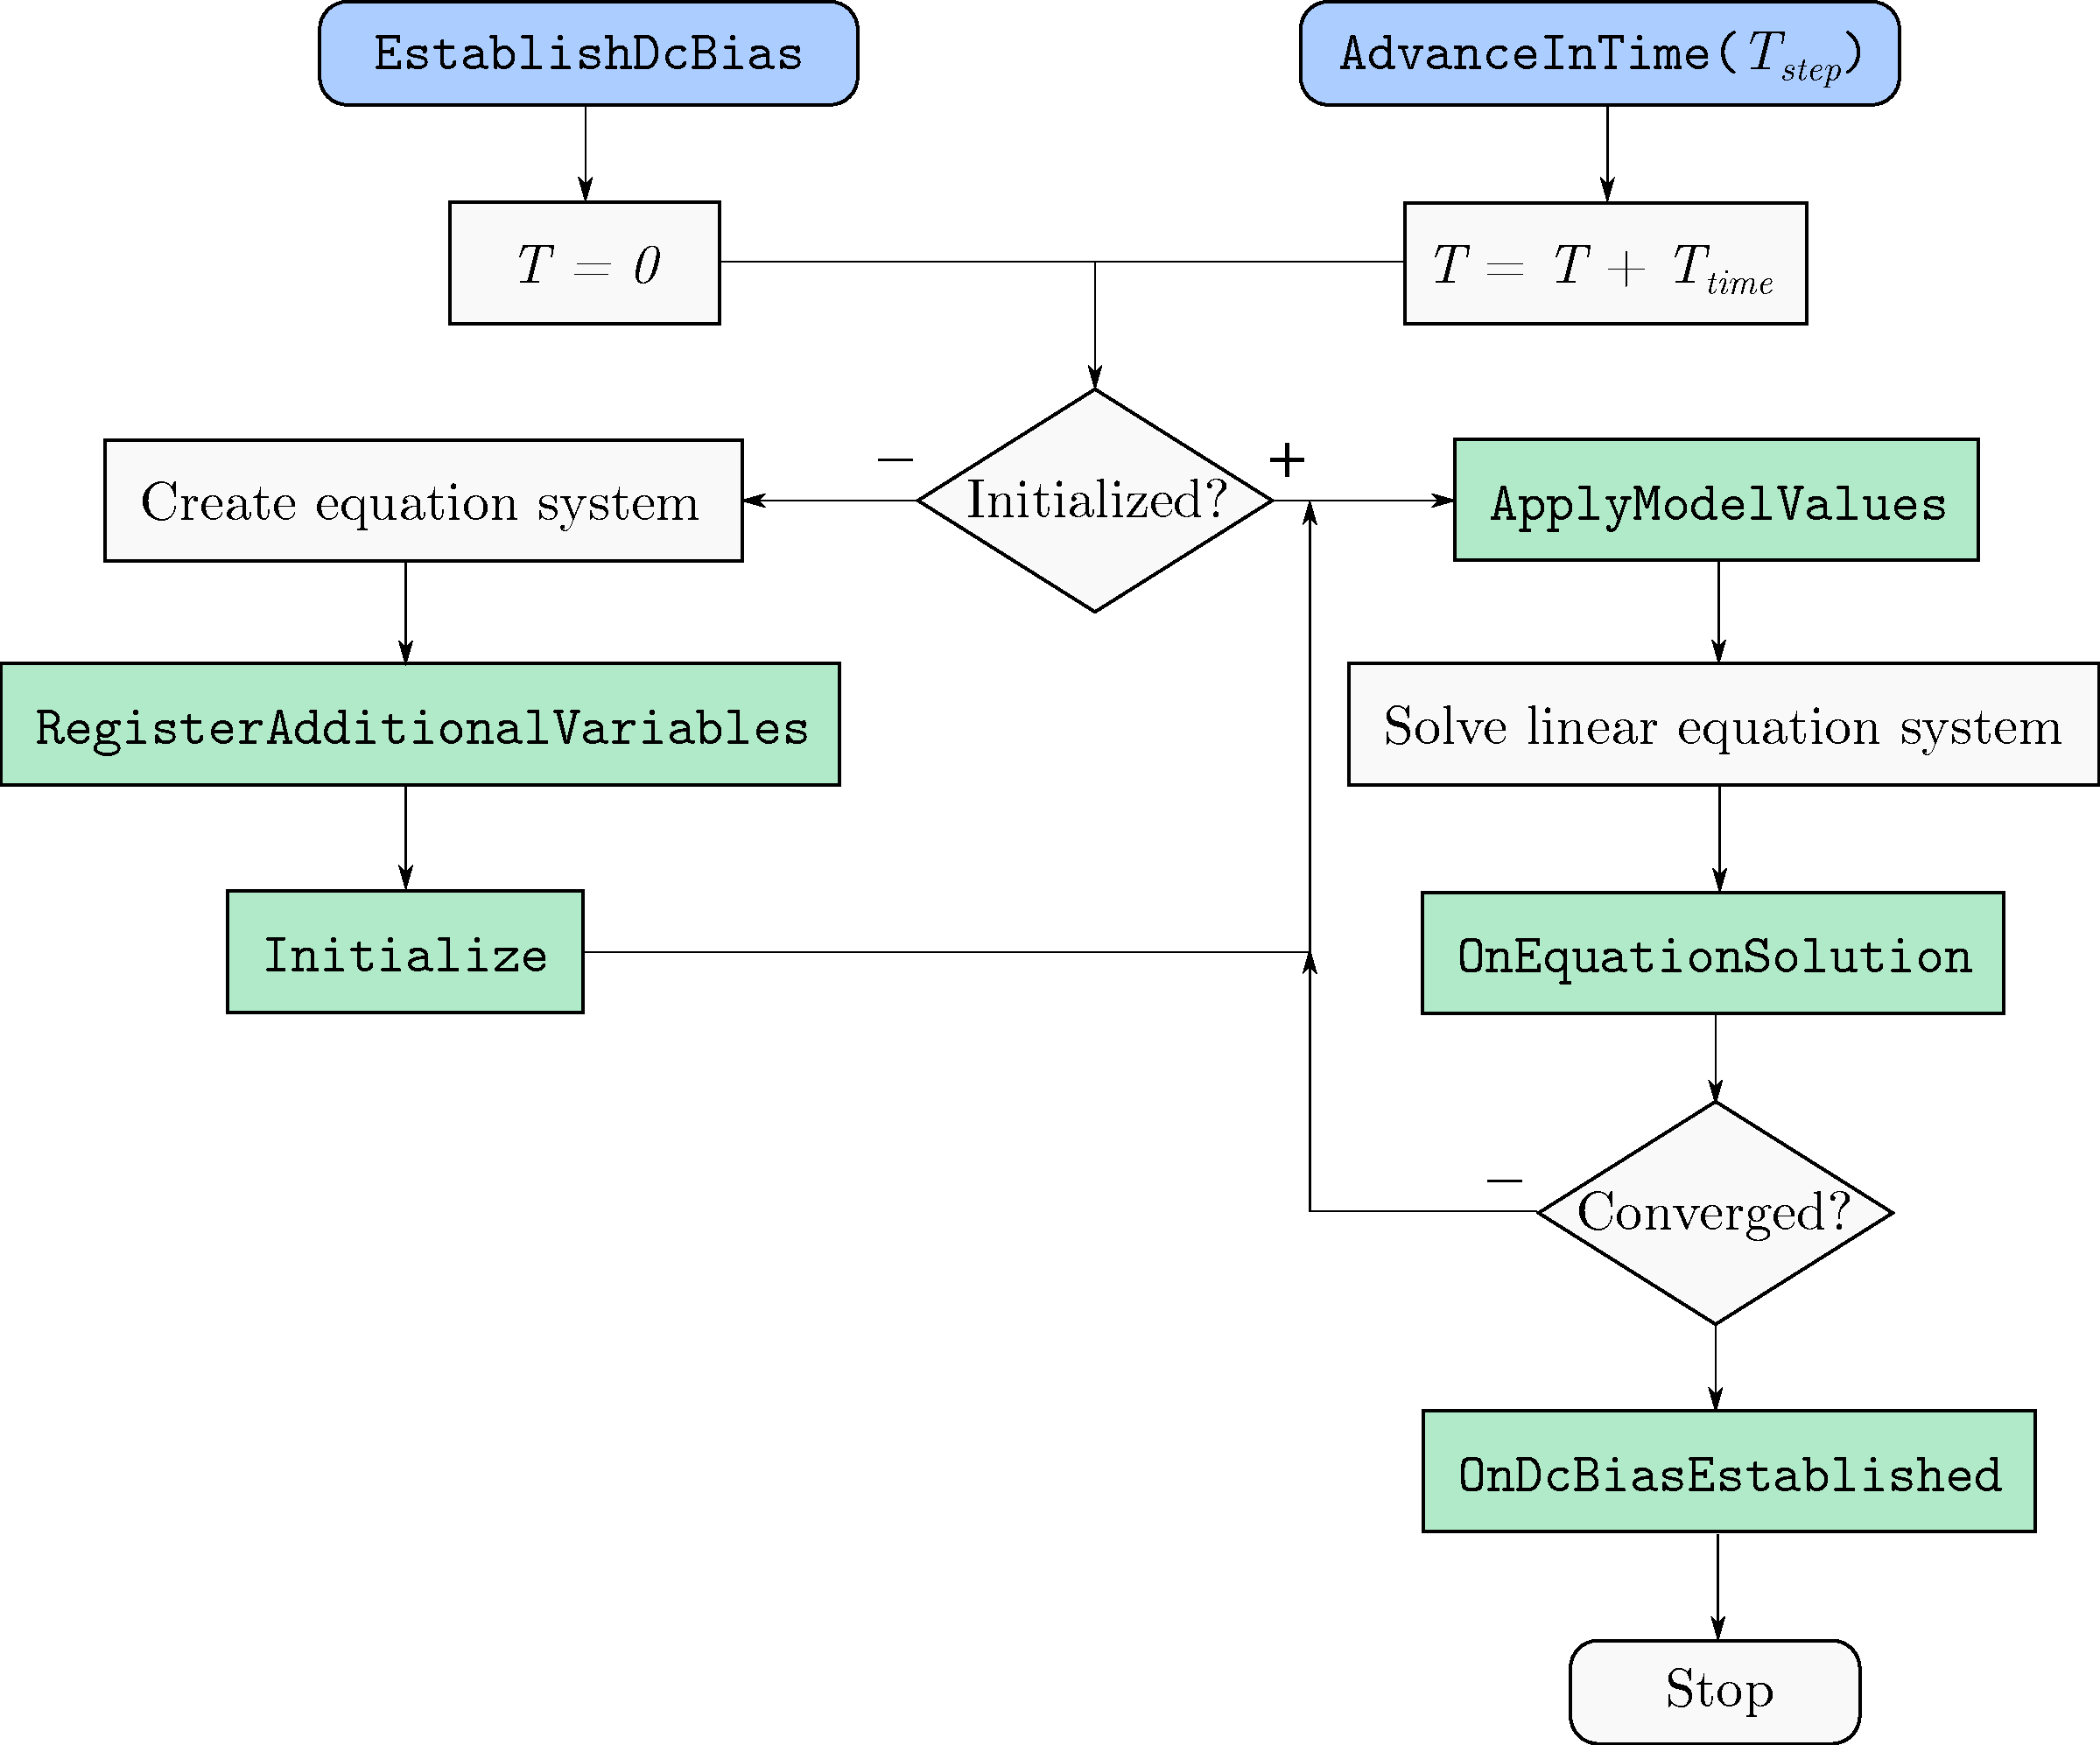
\includegraphics[width=\linewidth]{transient-analysis-implementation-diagram}
	\caption{Implementation of the simulation algorithm}
	\label{fig:transient-analysis-implementation-diagram}
\end{figure}

The following table lists the classes which implement the large-signal logic for individual circuit devices, and the corresponding section in QUCS Technical papers which describes the stamps and mathematical models used in the implementation. Also, the models for semiconductor devices (diode and BJT) are described in depth in Semiconductor Device Modeling with SPICE by G. Massobrio \cite{device_modeling}, ch 1 and 2.

\begin{center}
	\begin{tabular}{|l|l|}
		\hline
		Device class & QUCS section \\ \hline \hline
		\texttt{LargeSignalResistor} & 9.2 \\ \hline
		\texttt{LargeSignalCapacitor} & 6.3.1 \\ \hline
		\texttt{LargeSignalInductor} & 6.3.2 \\ \hline
		\texttt{LargeSignalVoltageSource} & 9.18 \\ \hline
		\texttt{LargeSignalCurrentSource} & 9.18 \\ \hline
		\texttt{LargeSignalVccs} & 9.20.1 \\ \hline
		\texttt{LargeSignalCccs} & 9.20.2 \\ \hline
		\texttt{LargeSignalVcvs} & 9.20.3 \\ \hline
		\texttt{LargeSignalCcvs} & 9.20.4 \\ \hline
		\texttt{LargeSignalDiode} & 10.2 \\ \hline
		\texttt{LargeSignalBjt} & 10.4 \\ \hline
	\end{tabular}
\end{center}

The actual stamping is delegated to \texttt{<device>Stamper} classes to make the implementation cleaner. 

\section[NextGenSpice.Numerics and NextGenSpice.Numerics.Native]{NextGenSpice.Numerics and \\ NextGenSpice.Numerics.Native}

\texttt{NextGenSpice.Numerics.Native} is the only C++ project in the solution. It is used to build a dynamically linked library, which contains the implementation of QD library used by NextGen SPICE for the double-double and quad-double precision types. It also contains a native implementation of the Gaussian elimination algorithm for solving the equation system to speed up the the simulation (see analysis section~\ref{chap:analysis:dd}).

\texttt{NextGenSpice.Numerics} is the managed counterpart of the \texttt{NextGenSpice\+.Numerics.Native} project. It contains C\# wrappers around the \texttt{dd\_real} and \texttt{qd\_real} types from QD library, with PInvoke calls to its exported methods. It also contains the managed implementation of Gaussian-elimination that is used when the library is compiled without the conditional compilation symbols mentioned at the beginning of this chapter.

\subsection{Equation System Implementation}
The \texttt{NextGenSpice.Numerics} project contains implementations of the equation system. There is a separate class for the equation system for each precision type: \texttt{EquationSystem}, \texttt{DdEquationSystem} and \texttt{QdEquationSystem}. These classes represent an equation system as a full matrix and vectors. To make the interface independent of the implementation and the actual precision type used, the equation system is exposed through the implementations of \texttt{IEquationSystem\+Adapter} and \texttt{IEquationSystemAdapterWide} interfaces. The first interface defines methods for getting proxies for individual equation system coefficients and the equation solution as described in the analysis chapter in section~\ref{chap:analysis:equation}. This interface will be exposed to the device's implementation. The other interface defines other methods that the simulator needs, like \texttt{Solve} and \texttt{Clear}. The actual implementation of these interfaces is requested from the static class \texttt{EquationSystemAdapterFactory}. This arrangement was chosen mainly to allow runtime changes of precision type for benchmarking purposes.

If the implementation were to change to a sparse matrix representation, then all that needs to be done is implementing the \texttt{IEquatioSystemAdapterWide} interface and replacing the class instantiated in the \texttt{EquationSystemAdapterFactory}.

\section{NextGenSpice}
This project contains the implementation of the standalone SPICE-like console application. This application directly uses the other parts of the NextGen SPICE library described in the preceding sections. This project implements necessary statement processors to handle \texttt{.PRINT}, \texttt{.OP} and \texttt{.TRAN} statements in the input netlist files. These statements are inserted into the \texttt{OtherStatements} collection on the \texttt{ParsingContext} and later retrieved from the property of same name on the \texttt{SpiceNetlistParserResult} object. If no error occurs while parsing the netlist, the application executes the requested simulations and prints the results on standard output.

\section{SandboxRunner}
This project serves only development purposes and is not deployed as part of the library. This project uses the BenchmarkDotNet NuGet package to run benchmarks for comparing the individual precision methods. It also contains examples of code which uses the library.

\section{Unit Test Projects}
There are three unit test projects in the solution, \texttt{NextGenSpice.Core.Test} for the core simulation library, \texttt{NextGenSpice.Parser.Test} for the parser and \texttt{NextGenSpice.LargeSignal.Test} for the large-signal simulations. These project use the XUnit NuGet package to run unit tests for the main parts of the tested projects. The unit tests do not aim for strict 100\% code coverage (The coverage is around 80\% for each project), instead, they test the most important parts of the library to avoid breaking the code when implementing new features in the library.
